\section{Network security protocols}

\paragraph*{Issues of communications security}
Communications security faces several challenges. 
Firstly, problems of remoteness include the need to establish trust between parties, protect sensitive data, and ensure the atomicity of transactions, meaning that each transaction must be complete and accurate. 
Internet protocols also present issues, particularly around authentication and confidentiality. 
Additionally, there is the transparency and critical mass problem, which involves ensuring that security protocols are widely adopted and consistently used.

\paragraph*{Secure protocols}
Two notable protocols that have addressed these challenges are HTTPS (HTTP over SSL/TLS) and SET (Secure Electronic Transaction). 
HTTPS ensures communication confidentiality and integrity, and allows for mutual authentication.
However, it does not guarantee how data is used and often does not strictly authenticate clients in practice. 
SET, developed by the VISA and MasterCard consortium, focused on securing transactions rather than connections, ensuring data usage and transaction security. 
Despite these strengths, SET failed to achieve critical mass and widespread adoption.

\subsection{Transport Layer Security}
SSL, originally designed by Netscape to secure web communication, became a de facto standard and evolved into TLS, standardized by the IETF. 
TLS, which succeeded SSL v3 and is currently at version 1.3, ensures the confidentiality and integrity of communications, server authentication, and optional client authentication. 
It uses both symmetric and asymmetric cryptography to balance performance and security. Versions up to TLS 1.1 are now considered insecure.
The TLS handshake involves several steps to establish a secure connection:
\begin{itemize}
    \item Client hello: the client sends a list of supported cipher suites and random data to the server.
    \item Server hello: the server responds with selected cipher suite, additional random data, and its certificate. 
        The client must verify the certificate.
    \item Key exchange: the client sends a pre-master secret encrypted with the server's public key and a client certificate signed with its private key.
    \item Secure communication: an encrypted communication channel is established.
\end{itemize}
TLS is designed to be flexible, supporting different suites of algorithms for key exchange, symmetric encryption, digital signatures, and hash functions. 
During the handshake, clients and servers compare cipher suites to agree on shared algorithms. 
This flexibility ensures that TLS can adapt to technical advancements.

TLS is inherently resistant to man in the middle attacks, as it ensures that only the legitimate parties involved in the communication can decrypt and modify the data.

\paragraph*{Summary}
TLS offers several benefits, including the protection of transmission confidentiality and integrity and the authentication of servers and, optionally, clients. 
However, it does not provide protection before or after transmission, such as on the server, client, or against abusers. 
Additionally, TLS relies on the Public Key Infrastructure (PKI), which introduces some limitations.

\subsection{Limitations and mitigations}
The effectiveness of TLS depends on the security and trustworthiness of root and intermediate Certificate Authorities (CAs). 
CAs are responsible for domain and organization validation and must meet specific requirements to be included in browser and OS root programs. 
Removing a non-compliant CA can disrupt many websites, making it a difficult decision.
To address some limitations, several mechanisms have been developed: 
\begin{itemize}
    \item HSTS (HTTP Strict Transport Security) uses an HTTP header to instruct browsers to always connect to a domain using HTTPS, with some browsers maintaining HSTS preload lists to enforce this. 
    \item  HPKP (HTTP Public Key Pinning), though now deprecated, allowed browsers to pin specific certificates or CAs to prevent trust issues from mis-issued certificates. 
    \item Certificate Transparency requires CAs to log metadata of issued certificates to an independent log, which browsers can enforce to defend against certificate mis-issuance.
\end{itemize}

\subsection{Secure Electronic Transaction}
SET was a collaborative effort by VISA and MasterCard to protect transactions rather than connections. 
The cardholder would send order details to the merchant and payment data to the payment gateway, which would verify the correspondence using a dual signature that linked the two pieces of a message directed to different recipients.
Despite its innovative approach, SET failed due to scalability issues, particularly the need for cardholders to obtain digital certificates, which hindered widespread adoption. 
Today, simpler methods, such as redirects with tokens to bank websites, are commonly used for secure transactions.
\begin{figure}[H]
    \centering
    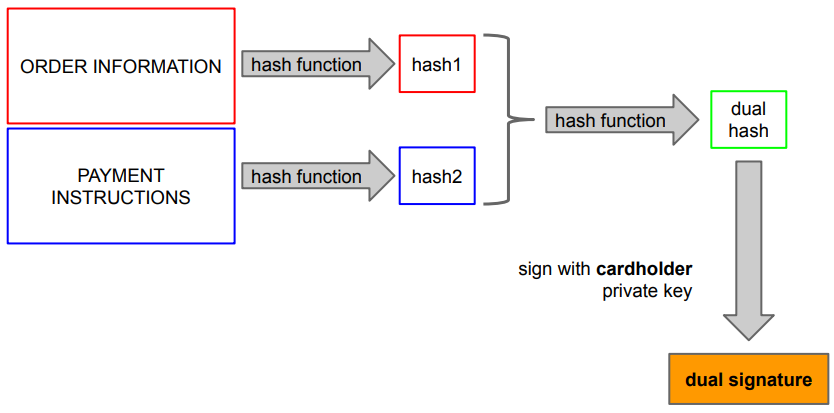
\includegraphics[width=1.0\linewidth]{images/dsg.png}
    \caption{Dual signature generation}
\end{figure}